\chapter{Mathematics}
\section{Geometry}

\subsection{Triangles}
Side lengths: $a,b,c$\\
Semiperimeter: $p=\dfrac{a+b+c}{2}$\\
Area: $A=\sqrt{p(p-a)(p-b)(p-c)}$\\
Circumradius: $R=\dfrac{abc}{4A}$\\
Inradius: $r=\dfrac{A}{p}$\\
Length of median (divides triangle into two equal-area triangles): $m_a=\tfrac{1}{2}\sqrt{2b^2+2c^2-a^2}$\\
Length of bisector (divides angles in two): $s_a=\sqrt{bc\left[1-\left(\dfrac{a}{b+c}\right)^2\right]}$\\
Law of sines: $\dfrac{\sin\alpha}{a}=\dfrac{\sin\beta}{b}=\dfrac{\sin\gamma}{c}=\dfrac{1}{2R}$\\
Law of cosines: $a^2=b^2+c^2-2bc\cos\alpha$\\
Law of tangents: $\dfrac{a+b}{a-b}=\dfrac{\tan\dfrac{\alpha+\beta}{2}}{\tan\dfrac{\alpha-\beta}{2}}$\\

\subsection{Quadrilaterals}
With side lengths $a,b,c,d$, diagonals $e, f$, diagonals angle $\theta$, area $A$ and
magic flux $F=b^2+d^2-a^2-c^2$:
 $$4A = 2ef \cdot \sin\theta = F\tan\theta = \sqrt{4e^2f^2-F^2} $$

 For cyclic quadrilaterals the sum of opposite angles is $180^\circ$,
$ef = ac + bd$, and $A = \sqrt{(p-a)(p-b)(p-c)(p-d)}$.

\subsection{Spherical coordinates}
\begin{center}
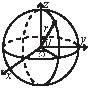
\includegraphics[width=25mm]{content/math/sphericalCoordinates}
\end{center}
\[\begin{array}{cc}
x = r\sin\theta\cos\phi & r = \sqrt{x^2+y^2+z^2}\\
y = r\sin\theta\sin\phi & \theta = \textrm{acos}(z/\sqrt{x^2+y^2+z^2})\\
z = r\cos\theta & \phi = \textrm{atan2}(y,x)
\end{array}\]


\section{Matrices}
    \kactlimport{Matrix.h}  
    \kactlimport{Determinant.h}
    \kactlimport{SolveLinear.h}
    \kactlimport{SolveLinearBinary.h}
    \kactlimport{MatrixInverse.h}

\section{FFT, Berlekamp}
    \kactlimport{FastFourierTransform.h}
    \kactlimport{NumberTheoreticTransform.h}
    \kactlimport{BerlekampMassey.h}
